\documentclass{report}

\usepackage[utf8]{inputenc}
\usepackage[francais]{babel} 
\usepackage{graphicx}
\usepackage[top=2cm, bottom=3cm, left=2.5cm, right=2.5cm]{geometry}%pour définir la taille des marges
\usepackage[justification=centering]{caption} %pour centrer le texte des légendes

\begin{document}

\section{Modification de la perspective}
L'image filmée par la caméra est vue de côté, cette étape de traitement a pour but de tranformer l'image initiale en une vue de dessus.

\subsection{Détection de points de réference sur le terrain}
La modification du point de vue de l'image nécessite la détection, sur l'image initiale, de la position de points de reference. Les points dont on va chercher à 
détecter la position sur l'image ont été entourés sur la figure~\ref{image_init}.

La détection va être réalisée en deux étapes :
\begin{itemize}
\item détection du plus long côté du tableau périodique (entouré en noir sur la figure~\ref{3droites}), prise de ses deux extrémités, qui sont les points \no 1 et 2
\item détection des deux petits côtés (entourés en rouge), puis calcule des points \no 3 et 4.
\end{itemize}

\begin{figure}[!h]
   \begin{minipage}[t]{.46\linewidth}
      \begin{center}
      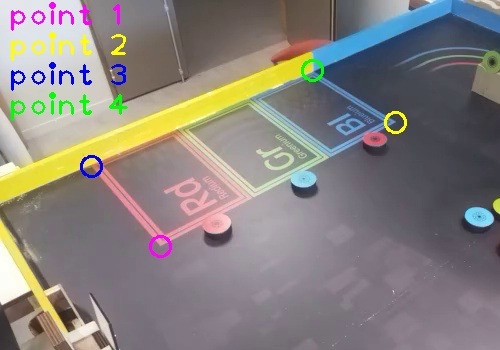
\includegraphics[height=150pt]{image_4_points.jpg}
      \end{center}
      \caption{Image filmée par la caméra du Raspberry Pi, les points recherchés ont été entourés}
      \label{image_init}
   \end{minipage} \hfill
   \begin{minipage}[t]{.46\linewidth}
      \begin{center}
      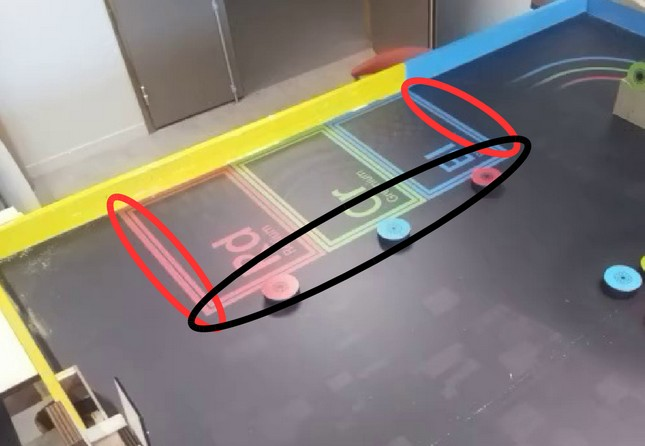
\includegraphics[height=150pt]{image_3_droites.jpg}
      \end{center}
      \caption{Les trois droites utilisées pour détecter les coins}
      \label{3droites}
   \end{minipage}
\end{figure}


\paragraph{Détection du long côté}
\subparagraph{Prise des contours}
L’application d’un filtre de Canny permet de mettre en évidence les contours présents dans l’image.
Le résultat de l’application de ce filtre est visible sur la figure~\ref{canny1}.
\begin{figure}[!h]
\begin{center} 
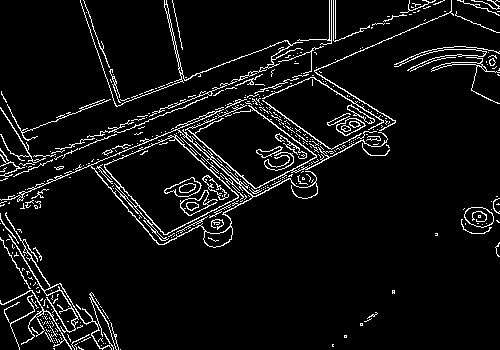
\includegraphics[height=130pt]{image_Canny.png}  
\end{center}
\caption{Résultat de l'application du filtre de Canny}
\label{canny1}
\end{figure}

\subparagraph{Détection de la droite}
La transformée de Hough détecte les droites présentes sur l’image. Cette fonction prend en argument un intervalle d’angle dans lequel rechercher des droites,
et le nombre minimum de pixels alignés pour qu’une droite soit détectée. Ces paramètres ont été choisi de manière à minimiser le nombre de droites détectées tout
en s’assurant que la droite recherchée ne soit pas ignorée. Les droites détectées par la transformée de Hough ont été tracées sur la figure~\ref{hough1}.

On recherche dans ces droites celle qui est la plus éloignée du coin en haut à gauche de l’image, elle a été tracée en violet.
\begin{figure}[!h]
\begin{center}
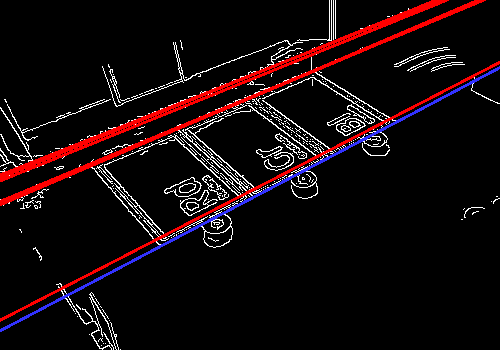
\includegraphics[height=130pt]{image_Canny_hough1.png}  
\end{center}
\caption{Résultat de la transformée de Hough, les droites détectés ont été tracés en rouge, et en bleu celle sélectionnée}
\label{hough1}
\end{figure}

\subparagraph{Détection des extrémités de cette droite}
La partie précédente a permis d’obtenir la droite recherchée, il faut maintenant en détecter les extrémités.

Un seuil de luminosité est appliqué à l’image initiale pour délimiter la zone du tableau périodique, sur la figure~\ref{seuillee} les pixels blancs
représentent les pixels de l’image ayant une luminosité suffisante. Pour une question de fiabilité, le seuil de luminosité qui est
appliqué n’est pas fixé par avance mais il est calculé à partir de la luminosité moyenne d’une partie de l’image où seul le fond gris
du tapis de jeu est visible.
Une opération « et logique » est ensuite appliquée entre la droite précédemment détectée et le résultat de l’opération de seuillage,
le résultat est donné sur la figure~\ref{droite1}. On récupère alors le plus long segment de cette image et on calcule la position de ses extrémités.

Cette première étape a permis de détecter deux coins du tableau périodique (les points 1 et 2 sur la figure~\ref{image_init}), ces points vont
faciliter la détection des deux petits côtés (encerclés en rouge sur la figure~\ref{3droites}).
\begin{figure}[!h] \hfill
   \begin{minipage}[t]{.4\linewidth}
      \begin{center}
      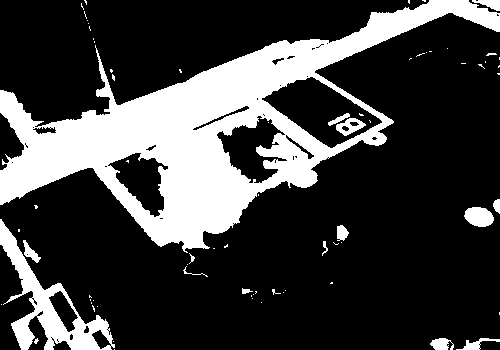
\includegraphics[height=130pt]{image_seuillee_en_luminosite.png}  
      \end{center}
      \caption{Image initiale seuillée en luminosité}
      \label{seuillee}
   \end{minipage} \hfill
   \begin{minipage}[t]{.4\linewidth}
      \begin{center}
      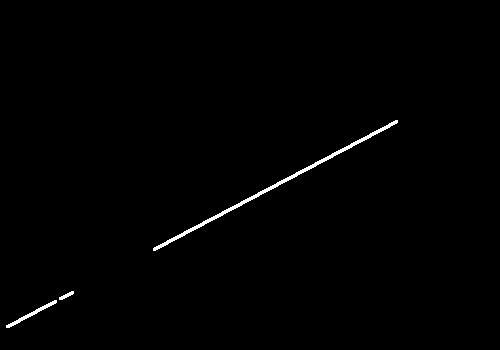
\includegraphics[height=130pt]{image_droite_1.png}  
      \end{center}
      \caption{Résultat de l'opération ``et logique'' entre l'image seuillée et la droite détectée}
      \label{droite1}
   \end{minipage} \hfill \hfill
\end{figure}

\paragraph{Détection des deux petits côtés}
\subparagraph{Détection de droites}
La transformée de Hough est à nouveau appliquée à l’image passée au filtre de Canny, avec des paramètres adaptés pour
les droites recherchées (voir figure~\ref{hough2}).
Pour chacun des points, on récupère la droite passant au plus près d’eux.
\begin{figure}[!h] \hfill
  \begin{minipage}[t]{.4\linewidth}
    \begin{center}
    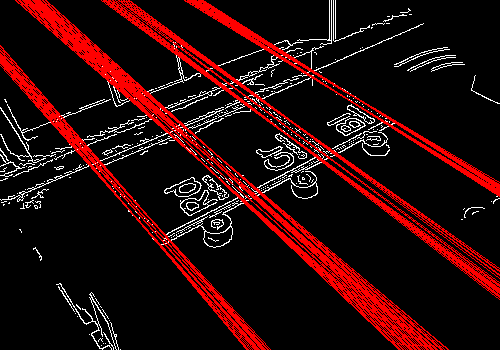
\includegraphics[height=130pt]{image_Canny_et_hough2.png}  
    \end{center}
    \caption{Résultat de la transformée de Hough}
    \label{hough2}
  \end{minipage} \hfill
  \begin{minipage}[t]{.4\linewidth}
    \begin{center}
    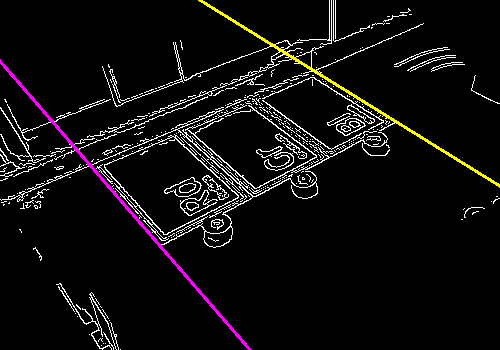
\includegraphics[height=130pt]{image_Canny_hough2_et_droites_choisies.png}  
    \end{center}
    \caption{Droites passant le plus près des deux points}
    \label{hough2bis}
  \end{minipage} \hfill\hfill
\end{figure}

\subparagraph{Calcul de la position des points \no3 et 4}
Les deux droites qui viennent d’être détectées donnent la direction du point \no1 vers le point 3, et du point \no2 vers le point 4,
on peut donc en déduire la position des points \no3 et 4

\subsection{Calcul d'une matrice de transformation de la perspective}
La position des points de reference obtenus précedemment va permettre de modifier le point de vue des images.

Une matrice de transformation de perspective est calculée telle que les quatre points sur l'image initiale se retrouvent
où ils seraient si le plateau de jeu avait été filmé en vue de dessus. En pratique, cette matrice est calculée pour que les points \no1 à 4
présent sur l'image de gauche de la figure~\ref{modif_perspective}, se retrouve aux points \no1' à 4' de l'image de droite.

\begin{figure}[!h]
\begin{center}
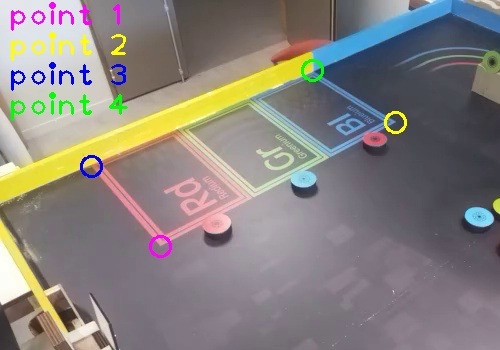
\includegraphics[height=130pt]{image_4_points.jpg}
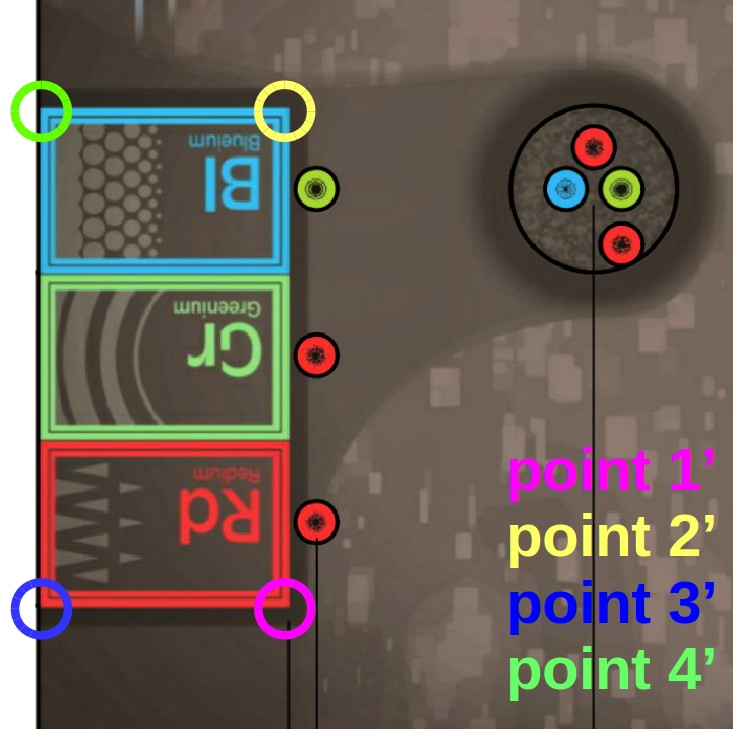
\includegraphics[height=130pt]{modif_perspective.jpg}
\end{center}
\caption{À gauche points détectés sur l'image initiale, à droite points d'arrivées entourés sur un schéma extrait du règlement de la coupe de France}
\label{modif_perspective}
\end{figure}

Cette matrice est ensuite appliquée à l'image intiale, le résultat est visible en figure~\ref{perspective_corrigee}

\begin{figure}[!h]
\begin{center}
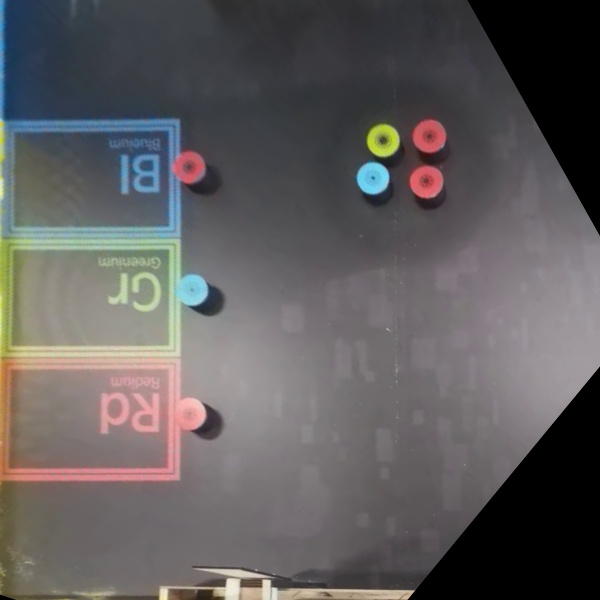
\includegraphics[height=150pt]{apres_modif_perspective.jpg}
\end{center}
\caption{Résultat de l'opération de modification de la perspective appliquée à l'image issue de la caméra}
\label{perspective_corrigee}
\end{figure}

\section{Détermination de la couleur des palets}
Afin de faciliter la détection des palets, leur couleur exacte est déterminée à partir de l'image initiale.
Les trois couleurs de palets (rouge, vert et bleu) sont les mêmes que les trois cases du tableau périodique, c'est donc la couleur des ces cases
qui est extraite car leur position est connue.

\paragraph{Extraction d'un échantillon de la couleur de chaque case du tableau périodique}
Les points \no1 et 2 sont utilisés pour extraire trois petites images contenant chacune une seule couleur.
L'échantillon de couleur rouge est extrait au voisinage du point \no1, celui de couleur bleue au voisinage du point \no2
et l'échantillon de couleur verte est extrait au voisinage du milieu du segment reliant les deux points.
Ces échantillons sont visible en figure~\ref{couleurs}.

\begin{figure}[!h]
\begin{center}
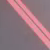
\includegraphics[height=70pt]{rouge_init.png}

\includegraphics[height=35pt]{vert_init.png}

\includegraphics[height=70pt]{bleu_init.png}
\end{center}
\caption{Échantillon des trois couleurs de palets}
\label{couleurs}
\end{figure}

\paragraph{Calcule de la valeur moyenne de couleur de chaque image}
Pour ces trois images, un seuillage en luminosité est appliqué afin de ne conserver que les pixels suffisamment lumineux.
Les pixels qui ne seront pas utilisés pour calculer la valeur moyenne de couleur ont été remplacés par des pixels noirs.
La valeur moyenne de couleur des pixels restants est calculée pour ces trois images.
\begin{figure}[!h]
\begin{center}

\includegraphics[height=70pt]{rouge_seuillee.png}

\includegraphics[height=35pt]{vert_seuillee.png}

\includegraphics[height=70pt]{bleu_seuillee.png}
\end{center}
\caption{Échantillon des trois couleurs de palets après seuillage}
\label{couleurs_seuillee}
\end{figure}

\end{document}